\documentclass[11pt,a4paper]{article}

\usepackage[a4paper,margin=2.0cm]{geometry}
\usepackage[T1]{fontenc}
\usepackage{lmodern}
\usepackage{amsmath,amssymb}
\usepackage{booktabs}
\usepackage{graphicx}
\usepackage{xcolor}
\usepackage[hidelinks]{hyperref}
\usepackage{fancyvrb}
\DeclareUnicodeCharacter{2229}{\ensuremath{\cap}}
\fvset{fontsize=\scriptsize,numbers=left,numbersep=4pt,frame=lines,framesep=2mm}

\graphicspath{{../figures/}}
% Small captions with a bold label, compact lists (without the caption/enumitem packages).
\makeatletter
\long\def\@makecaption#1#2{\vskip\abovecaptionskip{\small\textbf{#1.} #2\par}\vskip\belowcaptionskip}
\makeatother
\let\olditemize\itemize
\renewcommand{\itemize}{\olditemize\setlength{\itemsep}{1pt}\setlength{\parskip}{0pt}\setlength{\topsep}{2pt}}
\setlength{\parskip}{0.3em}
\setlength{\parindent}{0pt}

\newcommand{\npo}{NPO}
\newcommand{\xpo}{XPO}
\newcommand{\B}[1]{\textbf{#1}}

\title{\vspace{-1.6cm}Top-$N$ Group Recommendations with Fairness:\\
\large A Replication of Sacharidis (2019) and an Extension to Larger Groups}
\author{Luca Wunderer \and Felix Ries \and Marko Djordjevic \and Aleksa Slavkovic \and Taisiia Volynskaia\\[0.3em]
\small Applications of Data Science, WU Vienna \quad·\quad 22 November 2026\\
\small Code: \url{https://github.com/luwu5-bit/Applications-of-DataScience}}
\date{}

\begin{document}
\maketitle
\vspace{-1.2cm}

\begin{abstract}
\noindent
Sacharidis (2019) proposes two group recommenders, \npo{} and \xpo{}, which
recommend Pareto-optimal items and rank them by how often they reach the top~$N$
under random member weights. On MovieLens~1M the paper reports that \xpo{} is
far fairer to the worst-off group member than averaging (AVG). We reimplement
the method and all eight of the paper's methods, average every result over
20~matrix-factorization fits, and extend the group size from $m\le 8$ to $m=30$.
At the paper's main setting \xpo{} is the fairest method on every metric that
measures how much of each member's top~20 reaches the group list, but its lead
over AVG is a quarter to a half of the reported one. The lead shrinks with group
size and turns into a small AVG lead at 30~members, because \xpo{}'s pool can no
longer be narrowed. Under the paper's printed nDCG gain $2^{rel}$ no lead is
visible; we show that the paper's own numbers are inconsistent with that formula.
\end{abstract}

% =====================================================================
\section{Introduction}

A group recommender returns one top-$N$ list for $m$ people. Aggregating
predicted ratings by their mean (AVG) maximizes average satisfaction but can
leave one member with almost nothing they like. Sacharidis (2019) measures
\emph{fairness} as the utility of the worst-off member and proposes to
recommend only items that are not dominated in the members' rankings
(Pareto-optimal), ordered by how robustly they reach the top~$N$ when the
members are weighted at random. The paper reports large fairness gains over
AVG and least misery (LM), e.g.\ nDCG@20 fairness 0.406 for \xpo{} vs 0.298 for
AVG with five random users.

We (1)~replicate the paper's main experiment ($m=5$, $N=20$, random and
similar groups), (2)~extend it to groups of 2 to 30 members, tracking
fairness, utility, pool size and runtime, and (3)~explain where our numbers
differ, with every unspecified choice documented.

% =====================================================================
\section{Method}

\textbf{Setting.} For a group of $m$ users and a candidate set $C$ of 200
random movies, every member $u$ ranks $C$ by predicted rating; rank~1 is best.
The member's top~$N$ is their ground-truth list $\sigma_u$. Each item $i$
becomes a rank vector $r(i)=(r_{u_1}(i),\dots,r_{u_m}(i))$.

\textbf{Pareto pools.} Item $i$ dominates $j$ if $r_u(i)\le r_u(j)$ for all
members and $<$ for at least one. Let $d(i)$ be the number of items dominating
$i$. \npo{} uses the pool $\{i: d(i)\le N-1\}$, which provably contains every
item that can enter the top~$N$ under some linear weighting of the members.
\xpo{} uses the smallest level $x\in[1,N]$ such that
$|\{i: d(i)\le x-1\}|\ge N$, i.e.\ the tightest pool that still fills a list.

\textbf{Monte Carlo ranking.} We draw $S$ weight vectors $w$ from the simplex.
For each, the score $\sum_u w_u\,r_u(i)$ (lower is better) defines a top~$N$,
and each pool item in it gets a vote. The group list is the $N$ pool items with
the most votes.

\textbf{Baselines.} As in the paper: AVG (mean rating), LM (minimum rating),
MUL (product), MAX (maximum), BORDA (mean rank) and MED (median rank). As our
extension we add \emph{average without misery} (AWM; Masthoff, 2011): AVG
restricted to items no member rates below~3.

\textbf{Metrics.} A member's utility compares the group list $\sigma$ with
$\sigma_u$. \emph{Fairness} is the minimum over members, \emph{group utility}
the mean. We use P@$k$, AP and nDCG@$k$ as defined in the paper: the item at
position $p$ of $\sigma_u$ has relevance $rel=N-p+1$ (0 if absent) and the
discount is $\log_2(\text{pos}+1)$. The paper prints the gain $2^{rel}$. Under
this gain a member's favourite is worth $2^{19}$ times their 20th item and
alone accounts for about two thirds of the ideal DCG, so nDCG@20 essentially
asks whether each member's single favourite is near the top. Since the paper's
reported values are not consistent with this gain (Section~\ref{sec:paper}),
we report nDCG@20 with both the printed gain and the \emph{linear} gain $rel$.
As a further extension, two rating-based utilities capture what top-$N$
metrics cannot see, namely disliked items: the \emph{no-misery share} (share of
the list the member rates $\ge 3$) and the member's mean rating of the list.

% =====================================================================
\section{Experimental setup}

\textbf{Data and predictions.} MovieLens~1M (6{,}040 users, 3{,}706 rated
movies, 1.0M ratings). Missing ratings are filled by our own biased matrix
factorization trained with alternating least squares (50 factors,
regularization 0.06, 20 sweeps; test RMSE 0.852 on a 10\% hold-out).
Observed ratings are kept, predictions are clipped to $[1,5]$, as the paper
uses MF ``to fill in the missing ratings''.

\textbf{Random groups (RND)} are drawn uniformly without replacement.
\textbf{Similar groups (SIM)} follow the paper: ``starting from a randomly
selected user, the group is built incrementally by adding the most similar (in
terms of mean-centered cosine similarity) user''. As in the course (Unit~4,
after Baltrunas et al., 2010), groups are thus simulated from individual
ratings, with preference similarity as the proxy for cohesiveness. Each user
is a vector over all movies of their ratings minus their own mean (0 if
unrated); similarity is the cosine of two such vectors (Aggarwal, 2016,
Ch.~2). Centering removes the difference between generous and strict raters,
so users are similar when they like and dislike the same movies
\emph{relative to their own scale}. From a random seed user we repeatedly add
the user with the highest mean similarity to all current members. Ours, as
the paper is silent: the mean as similarity to a group, and all movies rather
than co-rated ones, which avoids spurious $\pm1$ similarities from one or two
shared movies (the course instead requires $\ge5$ co-rated films). The groups
are clearly homogeneous: at $m=5$ the mean pairwise similarity is 0.22 against
0.02 for random groups (more than 99\% of random pairs), and two members share
46\% instead of 36\% of their ground-truth top~20 (0.18 similarity at $m=30$).
A side effect: SIM favours users with many ratings (189 vs.\ 164 at $m=5$).

\textbf{Protocol.} 100 groups per setting, each with its own 200 candidates;
$S=10{,}000$ uniform (Dirichlet(1)) weight vectors; equally rated movies share
their average rank. The paper reports results for one prediction matrix, but
a single MF fit moved fairness by up to 0.03 in our checks, so \emph{every
experiment is run on 20~MF fits} that differ only in their random start. Per
group, a method's value is averaged over the fits; we report the mean over the
100 groups with 95\% confidence intervals over groups, and count in how many
fits a paired difference is significant on its own. From 15 to 20 fits no
setting mean moves by more than 0.002. All 20 assumptions are justified in
\texttt{ASSUMPTIONS.md}; none was tuned towards the paper's numbers.

% =====================================================================
\section{Results}

\subsection{Replication at five members}

\begin{table}[t]
\centering\footnotesize
\setlength{\tabcolsep}{3.4pt}
\begin{tabular}{l cccc c cccc}
\toprule
 & \multicolumn{4}{c}{Random groups (RND)} && \multicolumn{4}{c}{Similar groups (SIM)}\\
\cmidrule{2-5}\cmidrule{7-10}
 & nDCG lin & nDCG $2^{rel}$ & P@20 & paper nDCG && nDCG lin & nDCG $2^{rel}$ & P@20 & paper nDCG\\
\midrule
AVG   & 0.414 & 0.196 & 0.395 & 0.298 && 0.569 & 0.331 & 0.512 & 0.437\\
LM    & 0.316 & 0.092 & 0.309 & 0.197 && 0.452 & 0.211 & 0.419 & 0.403\\
MUL   & 0.411 & 0.183 & 0.393 & 0.290 && 0.565 & 0.320 & 0.509 & 0.438\\
MAX   & 0.317 & \B{0.260} & 0.316 & 0.208 && 0.420 & \B{0.362} & 0.405 & 0.329\\
BORDA & 0.401 & 0.135 & 0.385 & 0.210 && 0.552 & 0.271 & 0.496 & 0.203\\
MED   & 0.398 & 0.149 & 0.397 & 0.211 && 0.539 & 0.293 & 0.511 & 0.154\\
\npo  & 0.397 & 0.134 & 0.392 & 0.311 && 0.550 & 0.266 & 0.504 & 0.472\\
\xpo  & \B{0.460} & 0.203 & \B{0.414} & \B{0.406} && \B{0.606} & 0.332 & \B{0.516} & \B{0.579}\\
\midrule
AWM (ext.) & 0.408 & 0.184 & 0.389 & -- && 0.562 & 0.321 & 0.505 & --\\
\bottomrule
\end{tabular}
\caption{Fairness at $m=5$, $N=20$: mean over 100 groups and 20 MF fits
(95\% CIs $\pm0.015$ to $\pm0.033$). ``paper nDCG'': Sacharidis (2019),
Tables~1--2. Bold: fairest method per column.}
\label{tab:e1}
\end{table}

\begin{table}[t]
\centering\footnotesize
\setlength{\tabcolsep}{3.4pt}
\begin{tabular}{l ccccc c ccccc}
\toprule
 & \multicolumn{5}{c}{RND} && \multicolumn{5}{c}{SIM}\\
\cmidrule{2-6}\cmidrule{8-12}
 & nDCG lin & $2^{rel}$ & P@20 & AP & paper && nDCG lin & $2^{rel}$ & P@20 & AP & paper\\
\midrule
\xpo{} -- AVG & \B{+0.046} & +0.006 & \B{+0.018} & \B{+0.027} & +0.108 && \B{+0.037} & +0.001 & +0.004 & \B{+0.019} & +0.142\\
\xpo{} -- \npo{} & \B{+0.063} & \B{+0.068} & \B{+0.022} & \B{+0.021} & +0.095 && \B{+0.056} & \B{+0.066} & \B{+0.012} & \B{+0.017} & +0.107\\
\npo{} -- AVG & \B{$-$0.017} & \B{$-$0.062} & $-$0.003 & +0.006 & +0.013 && \B{$-$0.019} & \B{$-$0.065} & \B{$-$0.007} & +0.003 & +0.035\\
AWM -- AVG & \B{$-$0.006} & \B{$-$0.012} & \B{$-$0.006} & \B{$-$0.003} & -- && \B{$-$0.007} & \B{$-$0.011} & \B{$-$0.007} & \B{$-$0.006} & --\\
\bottomrule
\end{tabular}
\caption{Paired fairness differences at $m=5$ (mean over groups of the per-group
difference, averaged over 20 fits). Bold: 95\% CI excludes 0 (half-widths
0.003--0.012). \xpo{}--AVG under linear nDCG and AP is significant on each of
the 20 fits alone; under $2^{rel}$ on at most one. ``paper'': nDCG@20.}
\label{tab:diff}
\end{table}

\textbf{The paper's main claim holds in direction.} Under every metric that
counts how much of each member's top~20 reaches the group list---nDCG with
linear gain, P@20 and AP---\xpo{} is the fairest of all nine methods in random
groups, and under linear nDCG and AP also in similar groups. The lead over AVG
under linear nDCG (+0.046 RND, +0.037 SIM) is significant on each of the 20 MF
fits. \xpo{} beats \npo{} everywhere, and LM is among the least fair methods,
as in the paper. Under linear gain the ordering of the eight methods agrees
well with the paper's (Spearman $\rho=0.74$ RND, 0.60 SIM).

\textbf{It does not hold in size.} Our \xpo{}--AVG gap is about 40\% (RND) and
25\% (SIM) of the reported one under linear nDCG, and a fifth under P@20 (paper
+0.109 RND). \npo{} is slightly \emph{below} AVG, where the paper has it
slightly above. The levels differ as well: our baselines are about 0.1 above
the paper's values under linear nDCG, our \xpo{} 0.05 above. BORDA and MED are
far below AVG in the paper's SIM results (0.20 and 0.15 vs 0.44), which no
other method shows and which we do not reproduce.

\textbf{The printed gain hides the effect.} With gain $2^{rel}$, \xpo{} and AVG
are level (+0.006, +0.001) and MAX is the fairest method, because it places
93\% of the members' personal favourites in the list (AVG: 74\%), and with
$2^{rel}$ the favourite alone decides most of a member's score. The paper has
MAX clearly \emph{below} AVG (0.208 vs 0.298); under linear gain we find the
same (0.317 vs 0.414). Together with the inconsistency in
Section~\ref{sec:paper}, we read this as evidence that the paper did not compute
nDCG with the gain it prints, and we treat the $2^{rel}$ results as a
robustness check rather than the headline. \xpo{}'s advantage is that it puts
more of every member's top~20 into the list, not that it gets each member's
first place right.

\subsection{Group size}

\begin{figure}[t]
\centering
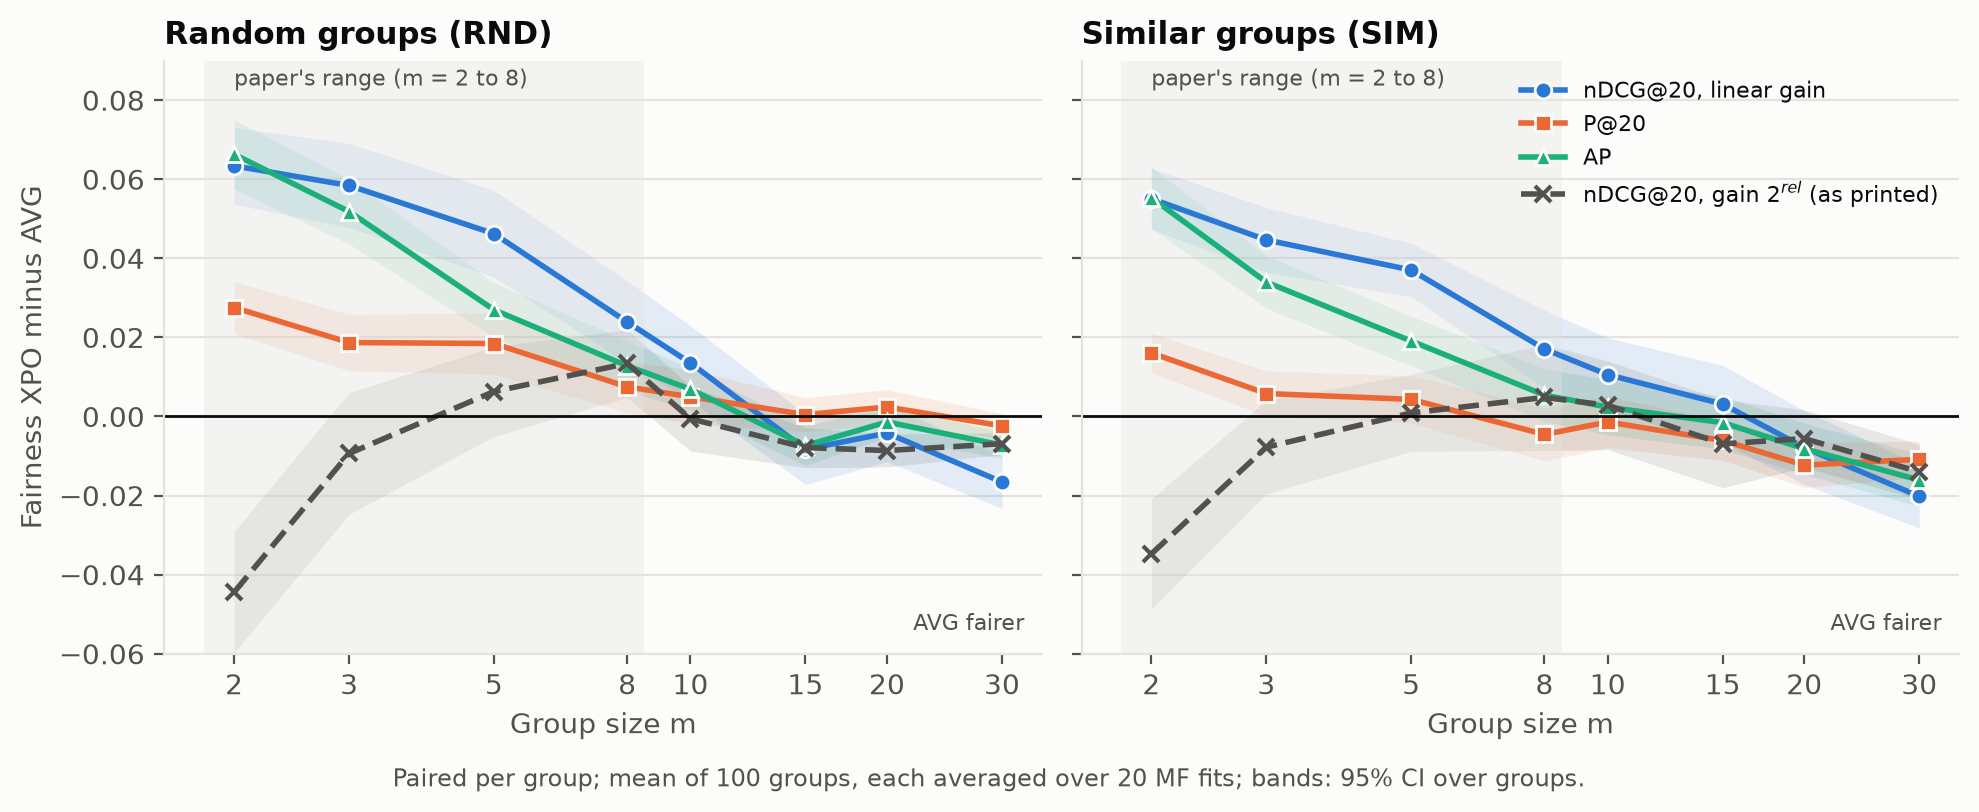
\includegraphics[width=\textwidth]{xpo_lead_by_metric.png}
\caption{Fairness of \xpo{} minus AVG by group size (E3; 100 groups per point,
20 MF fits). Above zero: \xpo{} is fairer. The shaded range is the one the paper
studies; $m=10$ to 30 is our extension.}
\label{fig:lead}
\end{figure}

\begin{figure}[t]
\centering
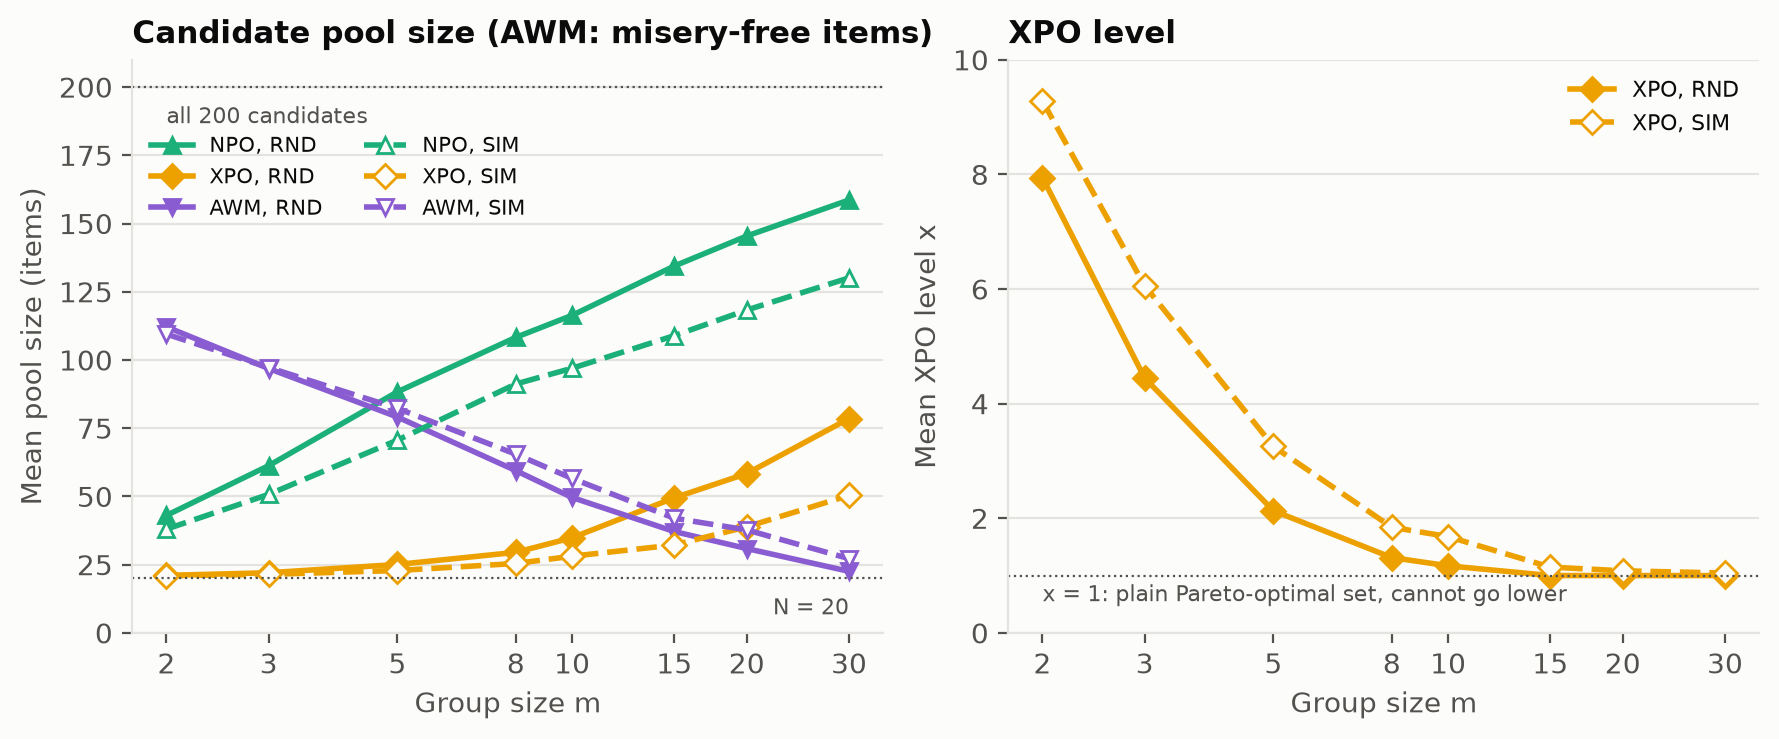
\includegraphics[width=0.74\textwidth]{pool_size_vs_group_size.png}
\caption{Left: candidate pool size of \npo{} and \xpo{} and number of
misery-free items (AWM). Right: mean \xpo{} level $x$. Level 1 is the plain
Pareto-optimal set and cannot be narrowed further.}
\label{fig:pool}
\end{figure}

Fairness falls quickly with group size for every method (linear nDCG, RND:
AVG 0.69 at $m=2$, 0.41 at $m=5$, 0.19 at $m=30$), and SIM groups stay above
RND groups, as in the paper. Figure~\ref{fig:lead} shows the central result of
the extension: \textbf{\xpo{}'s lead over AVG is largest for two or three
members and shrinks steadily with $m$}. The three coverage metrics agree on
this shape. Under linear nDCG the lead is significant on all 20 fits up to
$m=8$, vanishes around $m=15$, and at $m=30$ AVG is significantly fairer in
both group types ($-0.017$ RND, $-0.020$ SIM). Under the printed gain the curve
is flat around zero and even negative for pairs; its one positive point at
eight random members (+0.013) is significant on only 9 of 20 fits and is one of
16~cells, so we do not consider it a finding.

Figure~\ref{fig:pool} explains the decline. We expected that in large groups
almost every item becomes Pareto-optimal, so that \npo{}'s pool approaches all
candidates while \xpo{} stays selective. The first half holds partly: the
\npo{} pool grows from 22\% of the candidates at $m=2$ to 79\% at $m=30$ (SIM:
19\% to 65\%), and \npo{} stays below AVG at every size. The second half does
not hold: \xpo{}'s level $x$ falls from about 8 (RND) and 9 (SIM) at $m=2$ to 1
from $m=15$ on. At level~1 the pool is the plain Pareto set, which itself has
50 to 79 items in large random groups. \xpo{} then has nothing left to cut, and
\xpo{} and \npo{} become almost equally fair (linear nDCG at $m=30$, RND:
0.178 vs 0.176). Runtime is no concern (\npo{} 2--13\,ms, \xpo{} 0.7--8\,ms per group).

\subsection{Extension: disliked items and Average without Misery}

The paper's metrics only reward items in a member's top~20: an item outside
it scores zero whether the member rates it 4.5 or 1. Under the no-misery
share, the picture reverses. With five random members the worst-off member
dislikes one to one and a half of the 20 items under AVG (0.954) and \xpo{} (0.930), but
almost none under AWM (0.989) and LM (0.990). The gap grows with group size:
at $m=30$ AWM keeps the worst-off member's share at 0.88 against 0.76 for AVG
and \xpo{} (AWM--AVG +0.128, significant on all fits). In exchange AWM is
slightly below AVG on every top-$N$ metric (Table~\ref{tab:diff}), increasingly
so with $m$, because its misery-free set shrinks from 112 items at $m=2$ to 23
at $m=30$ (Figure~\ref{fig:pool}). \xpo{} is \emph{below} AVG on this metric for
$m\le15$: its pool is built from ranks only, so a movie one member hates is
Pareto-optimal as soon as another member loves it. Which method is ``fairest''
therefore depends on what fairness means: everyone gets some of their
favourites (\xpo{} for small groups), or nobody gets movies they dislike (AWM,
LM). The AWM threshold (3) and the rule for filling up a short list are our
choices; thresholds from 2 to 4 never made AWM fairer than AVG on the paper's
metrics by more than 0.001.

% =====================================================================
\section{Critical evaluation}

\subsection{Issues in the paper}\label{sec:paper}
\begin{itemize}
\item \textbf{nDCG does not fit the printed formula.} Under gain $2^{rel}$,
nDCG@1 is 1 only if the first group item is the member's favourite and halves
with every rank below, so it must lie far below P@1. The paper reports almost
equal values (AVG group utility: nDCG@1 0.694, P@1 0.702); with the printed
formula we obtain 0.280 vs 0.876. The printed gain is also unusual: the
standard form, as in the course (Unit~4), is $2^{rel}-1$.
\item \textbf{A results column is duplicated.} In both result tables,
fairness~P@1 equals group-utility~P@10 in every row.
\item \textbf{The toy example is miscalculated:} $i_2$ is top-1 with probability $3/5$, not $4/7$.
\item \textbf{Key settings are missing:} weight samples and distribution, MF
settings, ties, group similarity, significance tests.
\end{itemize}
Exact values therefore cannot be reproduced; we compare orderings and trends.

\subsection{Limitations of our replication}
\begin{itemize}
\item \textbf{Choices matter at the size of the effect.} In single-fit checks,
breaking rating ties by movie id instead of using tied ranks added about 0.02 to
\xpo{}'s lead under $2^{rel}$, because the same arbitrary order then decided
both \xpo{}'s ranks and the ground truth. Using MF predictions also where real
ratings exist raised all levels and gave \xpo{} leads of 0.02 to 0.03 under
$2^{rel}$, still far from the paper's 0.11 (checked under $2^{rel}$ only).
\item \textbf{Monte Carlo noise per group.} $S=10{,}000$ is enough on average
(means change by at most 0.002 up to $S=50{,}000$), but a single group's
fairness can still change by up to 0.23 when two items have nearly equal
votes.
\item \textbf{Scope.} One dataset, 100 groups per setting, $N=20$ only. The
ground truth is the members' \emph{predicted} top~20, so all methods are judged
by the same MF model that produces their inputs, as in the paper. We picked linear gain as the alternative to
$2^{rel}$; the paper's true gain is unknown.
\end{itemize}

% =====================================================================
\section{Conclusion}

We replicated the direction of Sacharidis (2019) but not its size: for small
groups \xpo{} is the fairest of nine methods on every coverage metric, by
roughly a third of the reported margin, and \npo{} does not improve on
averaging. Our extension shows that the advantage is a small-group effect: from
about 15 members on the Pareto set is too large for \xpo{} to narrow, and AVG is
as fair or fairer. If fairness means avoiding disliked items, a simple
average-without-misery rule beats all of the paper's methods.

\small
\section*{References}\vspace{-0.4em}
\begin{itemize}
\renewcommand{\labelitemi}{}
\item Aggarwal, C.\,C. (2016). \emph{Recommender Systems: The Textbook}. Springer.
\item Baltrunas, L., Makcinskas, T., \& Ricci, F. (2010). Group recommendations with rank aggregation and collaborative filtering. In \emph{Proc.\ 4th ACM Conference on Recommender Systems (RecSys '10)} (pp.\ 119--126).
\item Harper, F.\,M., \& Konstan, J.\,A. (2015). The MovieLens datasets: History and context. \emph{ACM Transactions on Interactive Intelligent Systems}, 5(4), 19:1--19:19.
\item Masthoff, J. (2011). Group recommender systems: Combining individual models. In \emph{Recommender Systems Handbook} (pp.\ 677--702). Springer.
\item Sacharidis, D. (2019). Top-N group recommendations with fairness. In \emph{Proc.\ 34th ACM/SIGAPP Symposium on Applied Computing (SAC '19)} (pp.\ 1663--1670). \url{https://doi.org/10.1145/3297280.3297442}
\end{itemize}

\textbf{Use of AI tools.} Claude Code (Anthropic) helped with code, diagnostics,
figures and draft text; all was checked by the team (log: \texttt{AI\_USE.md}).

% =====================================================================
\clearpage
\normalsize
\appendix
\section{Code}

The full project (Python~3.11, numpy/pandas) is in the repository linked on
the title page; this appendix prints the library code in \texttt{src/gfair/}
and the experiment driver. Plotting and summary scripts are only in the
repository. To reproduce all results, with MovieLens~1M in
\texttt{data/raw/ml-1m/}:
\begin{Verbatim}[numbers=none,frame=none,fontsize=\small]
pip install -r requirements.txt
python scripts/train_mf.py                      # RMSE check + prediction matrix
pytest -q                                       # 42 tests, incl. the Fig. 1 toy example
python scripts/run_experiment.py --exp E1       # 20 MF fits; likewise E2, E3, E5
python scripts/summarize.py && python scripts/make_figures.py
\end{Verbatim}

\newcommand{\code}[1]{\subsection*{\texttt{#1}}\VerbatimInput{../#1}}
\code{src/gfair/pareto.py}
\code{src/gfair/aggregators.py}
\code{src/gfair/metrics.py}
\code{src/gfair/groups.py}
\code{src/gfair/mf.py}
\code{src/gfair/data.py}
\code{src/gfair/config.py}
\code{src/gfair/experiment.py}
\code{scripts/run_experiment.py}

\end{document}
